\chapter{Risultati}
\label{ch:risultati}
\section{Differenze tra modello normale e compresso}
\label{sec:differenze modello normale e compresso}
Dati i problemi che comportavano l'utilizzo dei modelli da 4.8 GB, si è scelto di utilizzare per l'analisi dei risultati le versioni compresse da appena 20 MB ottenute tramite product quantization.
Per misurare la differenza di prestazioni tra il modello originale e la sua versione compressa si è considerato come riferimento il modello di Bijeeta et alii, avente le seguenti caratteristiche:
\begin{itemize}
    \item traduzione della sequenza dei tasti premuti con \texttt{word2keypress}
    \item numero minimo di n-gram pari a 1;
    \item numero di epoche di training pari a 5.
\end{itemize}
Per entrambi i modelli si è tenuto conto del valore di precision e recall, in modo da fornire una valutazione efficace del modello.
Non sono state osservate differenze significative riguardanti i valori, motivo per il quale si è scelto di considerare soltanto le versioni compresse per valutare gli altri modelli.

\begin{figure}[H]
    \centering
    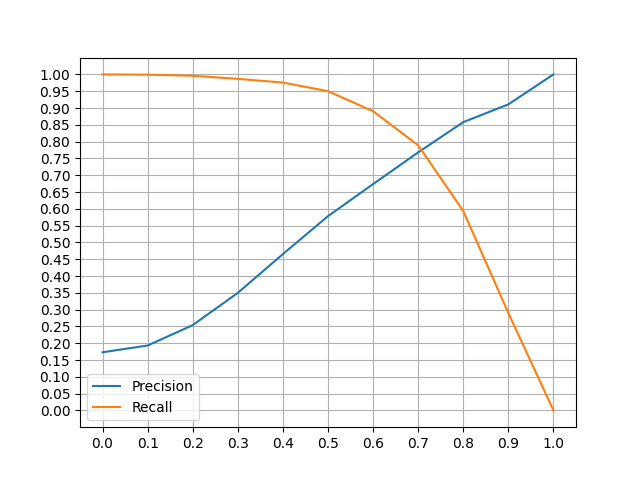
\includegraphics[width=11.5cm]{./immagini/big_model.png}
    \caption{Precision e recall nel modello non compresso di Bijeeta et al.~\cite{bijeeta} con le euristiche definite nel paragrafo \ref{sec:risultati euristiche adottate}, con \texttt{word2keypress}, \texttt{n\_mingram = 1},\\\texttt{epoche = 5}}
    \label{bigmodel}
\end{figure}

\begin{figure}[H]
    \centering
    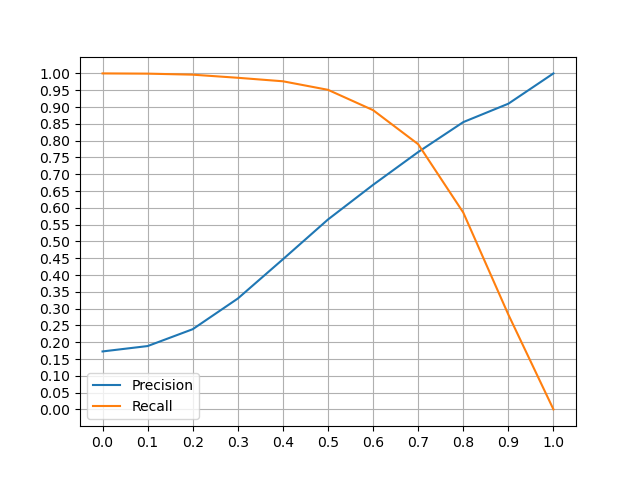
\includegraphics[width=11.5cm]{./immagini/CORRETTO_w2kp_nmingram=1_epochs=5.png}
    \caption{Precision e recall nel modello compresso di Bijeeta et al.~\cite{bijeeta} con le euristiche definite nel paragrafo \ref{sec:risultati euristiche adottate}, con \texttt{word2keypress}, \texttt{n\_mingram = 1},\\\texttt{epoche = 5}}
    \label{primomodello}
\end{figure}

\section{Classificazione del modello}
\label{sec:classificazione modello}
\subsection{Euristiche adottate}
\label{sec:risultati euristiche adottate}
Per valutare i modelli, a differenza di Bijeeta et alii~\cite{bijeeta}, non si è utilizzato Pass2Path a causa della complessa implementazione. Si è invece adottata la seguente euristica:
\begin{itemize}
    \item verifica della password con la variante minuscola;
    \item verifica della password con la variante maiuscola;
    \item verifica della password con la traduzione in codice \texttt{l33t};
    \item verifica se l'edit distance della password supera 5.
\end{itemize}

\subsection{Ground truth e prediction}
\label{sec:ground truth e prediction}
Per \emph{ground truth} si intende il risultato ideale che ci si aspetta e viene utilizzato per verificare una correttezza delle previsioni del modello.~\cite{lemoigne2008molecular}

Il termine \emph{prediction} si riferisce all'output di un modello dopo che è stato allenato su un dataset e applicato a nuovi dati quando si vuole prevedere la probabilità di un certo evento.~\cite{prediction}.

Per calcolare il valore di ground truth si tiene conto delle candidate due password e della euristica scelta; per ottenere il valore di prediction invece si considera si utilizza la funzione \texttt{gensim.similarity} del modello allenato, che sfrutta la cosine similarity discussa nel capitolo \ref{Similarita tra parole}.
Nel caso in cui si consideri la variante con \texttt{word2keypress} occorre convertire le due password in sequenza di tasti premuti prima di ricavare il valore di prediction.
\subsection{Precision e recall}
Per ricavare precision e recall si utilizza l'approccio di cui accennato nel paragrafo \ref{sec:classificazione password}; a questo scopo si definiscono i seguenti parametri:
\begin{itemize}
    \item \textbf{Veri positivi (TP)}: viene incrementato se sia la prediction che la ground truth hanno valore positivo non nullo;
    \item \textbf{Falsi positivi (FP)}: viene incrementato se la ground truth è nulla e la similarità è positiva non nulla;
    \item \textbf{Falsi negativi (FN)}: viene incrementato se la ground truth è positiva non nulla e la similarità è nulla;
\end{itemize}
Successivamente si ricava il valore di precision e recall nel seguente modo (cfr. paragrafo \ref{sec:classificazione password}):
\begin{gather*}
precision = \frac{TP}{TP + FP}
\\
recall = \frac{TP}{TP + FN}
\end{gather*}

\section{Similarità: un confronto}
\label{sec:similarita, confronto tra modelli}
In base a quanto spiegato nel paragrafo \ref{sec:classificazione password} si sono ottenuti i seguenti grafici:
\begin{figure}[H]
    \centering
    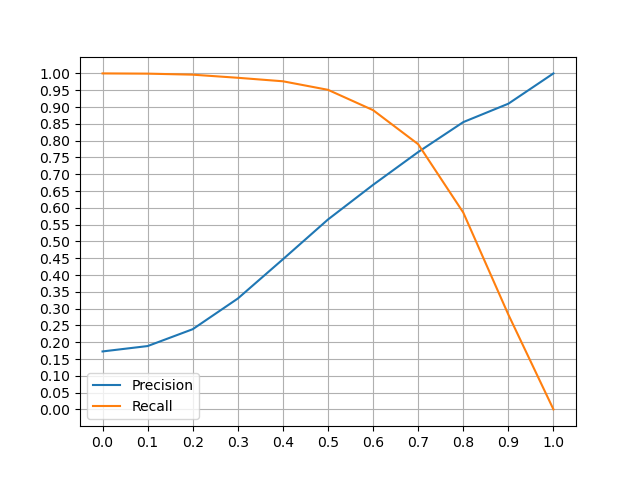
\includegraphics[width=14cm]{./immagini/CORRETTO_w2kp_nmingram=1_epochs=5.png}
    \caption{Precision e recall nel modello di Bijeeta et al.~\cite{bijeeta} con le euristiche definite nel paragrafo \ref{sec:risultati euristiche adottate}, con \texttt{word2keypress}, \texttt{n\_mingram = 1}, \texttt{epoche = 5}}
    \label{primomodello}
\end{figure}
\begin{figure}[H]
    \centering
    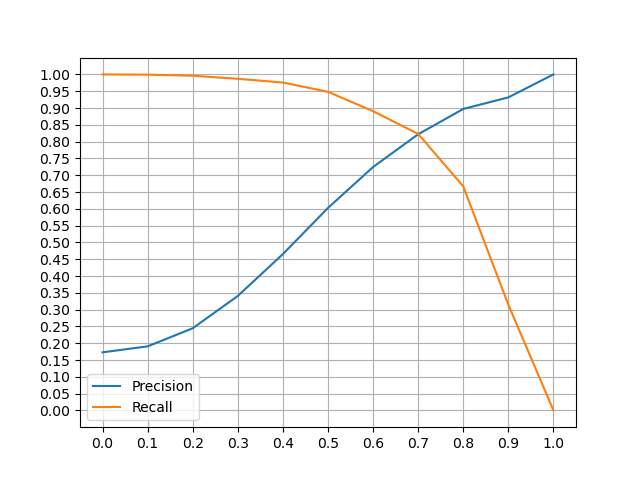
\includegraphics[width=14cm]{./immagini/no_w2kp_nmingram=1_epochs=5.png}
    \caption{Precision e recall nel modello senza \texttt{word2keypress}, \texttt{n\_mingram = 1}, \texttt{epoche = 5}}
    \label{secondomodello}
\end{figure}

\begin{figure}[H]
    \centering
    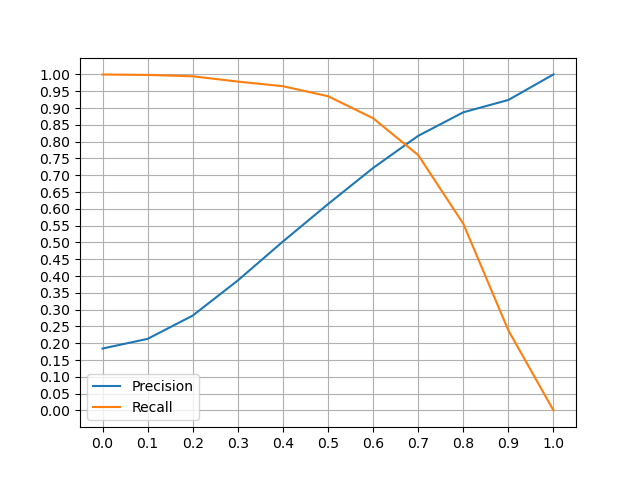
\includegraphics[width=14cm]{./immagini/CORRETTO_w2kp_nmingram=2_epochs=10.png}
    \caption{Precision e recall nel modello con \texttt{word2keypress}, \texttt{n\_mingram = 2}, \texttt{epoche = 10}}
    \label{terzomodello}
\end{figure}

\begin{figure}[H]
    \centering
    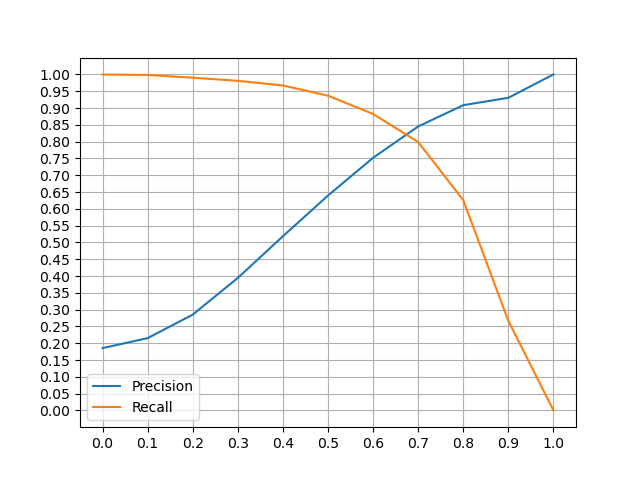
\includegraphics[width=14cm]{./immagini/no_w2kp_nmingram=2_epochs=10.png}
    \caption{Precision e recall nel modello senza \texttt{word2keypress}, \texttt{n\_mingram = 2}, \texttt{epoche = 10}}
    \label{quartomodello}
\end{figure}

\begin{figure}[H]
    \centering
    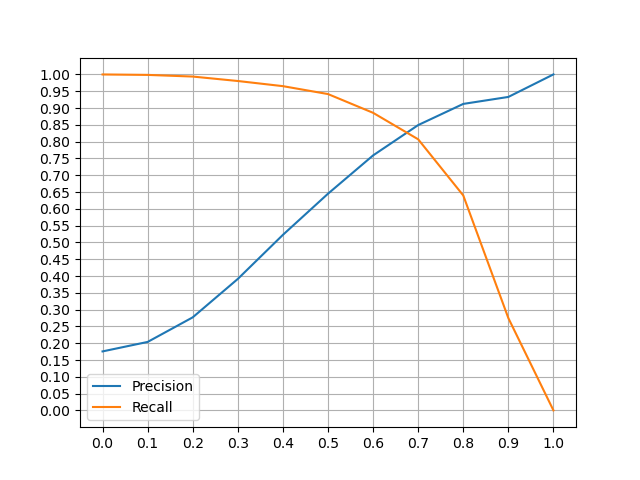
\includegraphics[width=14cm]{./immagini/no_w2kp_nmingram=2_epochs=5.png}
    \caption{Precision e recall nel modello senza \texttt{word2keypress}, \texttt{n\_mingram = 2}, \texttt{epoche = 5}}
    \label{quintomodello}
\end{figure}

\section{Risultati ottenuti}
\label{sec:risultati ottenuti}
Come accennato in \ref{sec:classificazione password}, per classificare le password è necessario definire una soglia $\alpha$ di similarità, in modo da definire due password simili tra loro se la loro similarità supera $\alpha$, diverse tra loro altrimenti.
Analizzando i modelli ottenuti, si possono osservare i seguenti risultati:
\begin{itemize}
    \item con \texttt{word2keypress}, \texttt{n\_mingram = 1}, \texttt{epoche = 5} (modello di Bijeeta et
    \\alii~\cite{bijeeta}, figura \ref{primomodello}):
    \begin{itemize}
        \item $\alpha = 0.5$: precision pari a $\simeq 57\%$ e recall pari a $\simeq 95\%$
        \item $\alpha = 0.6$: precision pari a $\simeq 67\%$ e recall pari a $\simeq 89\%$
    \end{itemize}
    \item senza \texttt{word2keypress}, \texttt{n\_mingram = 1}, \texttt{epoche = 5} (figura \ref{secondomodello}):
    \begin{itemize}
        \item $\alpha = 0.5$: precision pari a $\simeq 60\%$ e recall pari a $\simeq 95\%$
        \item $\alpha = 0.6$: precision pari a $\simeq 73\%$ e recall pari a $\simeq 88\%$
    \end{itemize}
    \item con \texttt{word2keypress}, \texttt{n\_mingram = 2}, \texttt{epoche = 10} (figura \ref{terzomodello}):
    \begin{itemize}
        \item $\alpha = 0.5$: precision pari a $\simeq 62\%$ e recall pari a $\simeq 94\%$
        \item $\alpha = 0.6$: precision pari a $\simeq 73\%$ e recall pari a $\simeq 87\%$
    \end{itemize}
    \item senza \texttt{word2keypress}, \texttt{n\_mingram = 2}, \texttt{epoche = 10} (figura \ref{quartomodello}):
    \begin{itemize}
        \item $\alpha = 0.5$: precision pari a $\simeq 65\%$ e recall pari a $\simeq 94\%$
        \item $\alpha = 0.6$: precision pari a $\simeq 75\%$ e recall pari a $\simeq 88\%$
    \end{itemize}
    \item senza \texttt{word2keypress}, \texttt{n\_mingram = 2}, \texttt{epoche = 5}
    (figura \ref{quintomodello}):
    \begin{itemize}
        \item $\alpha = 0.5$: precision pari a $\simeq 65\%$ e recall pari a $\simeq 95\%$
        \item $\alpha = 0.6$: precision pari a $\simeq 77\%$ e recall pari a $\simeq 89\%$
    \end{itemize}
\end{itemize}
I modelli con i migliori risultati non utilizzano la libreria \texttt{word2keypress}, e presentano un miglioramento di almeno il 3\% nel valore di precision e con valore di recall invariato, rispetto ai modelli che utilizzano \texttt{word2keypress}.

Un altro importante miglioramento è stato determinato dal valore di \texttt{n\_mingram}: tutti i modelli con \texttt{n\_mingram = 2} hanno avuto un lieve incremento del valore di precision.

Il modello con i risultati più scarsi è quello con \texttt{word2keypress}, \texttt{n\_mingram = 1}, \texttt{epoche = 5} (modello di Bijeeta et
alii~\cite{bijeeta}, figura \ref{primomodello}), e lo si può osservare dai valori inferiori di precision rispetto ad altri modelli.

Il modello con le migliori performance è invece riportato in figura \ref{quintomodello}, senza \texttt{word2keypress}, \texttt{n\_mingram = 2}, \texttt{epoche = 5}, con valore di precision pari a 77\%, per $\alpha = 0.6$, superiore di $\simeq 10\%$ rispetto al modello di Bijeeta et alii~\cite{bijeeta}.

\subsection{Criticità del modello proposto da Bijeeta et alii}
\label{sec:criticita bijeeta}
I motivi per cui il modello di Bijeeta et alii~\cite{bijeeta} è risultato il peggiore sono i seguenti:
\begin{itemize}
    \item La libreria \texttt{word2keypress} traduce ciascun carattere come sequenza di tasti premuti, come accennato nel paragrafo \ref{sec:allenamento pass2path}. Di conseguenza, quando si hanno due password che presentano un'alternanza di caratteri minuscoli e maiuscoli, esse risulteranno molto simili tra loro, a causa della ripetizione delle sequenze \texttt{<s> <c>}.
    \item Sempre a causa di \texttt{word2keypress}, la presenza di caratteri speciali non consecutivi che si ottengono premendo \texttt{SHIFT}, ad esempio:
    \begin{itemize}
        \item la password \texttt{\$1mp@t1c*}, che viene tradotta come \texttt{<s>41mp<s>2t1c<s>8})
        \item la password \texttt{\#wlng\%p*m\}} che viene tradotta come\\ \texttt{<s>3wlng<s>5p<s>8m<s>[}
    \end{itemize}
    rende la valutazione di similarità tra due password poco affidabile, poiché verrebbero valutate come simili, quando in realtà dovrebbero essere valutate come sicure e diverse tra loro.
    \item L'utilizzo di \texttt{n\_mingram = 1} rende la valutazione meno precisa rispetto allo stesso modello con \texttt{n\_mingram = 2}, poiché risulta più efficace valutare la vicinanza di due specifici bigrammi, anziché avere una valutazione maggiormente dispersiva in cui si considera la posizione di un carattere rispetto a un altro. Nelle password, infatti, risulta che i singoli caratteri non dipendano da un insieme di regole (come nel caso della letteratura inglese), ma vengano fortemente influenzati da fattori distinti tra loro e difficilmente rappresentabili.
\end{itemize}

\subsection{Soglia di similarità per la valutazione di due password}
\label{sec:soglia similarita valutazione due password}
Per potere determinare se due password siano simili tra loro occorre definire la soglia di similarità $\alpha$, tenendo in considerazione i valori di precision e recall ottimali.

Nel caso in studio, è necessario avere un valore di recall più alto rispetto al valore di precision, dato che è importante rilevare più password simili tra loro possibili. Questo tuttavia, per valori di precision molti bassi (come accennato nel paragrafo \ref{sec:classificazione password}) può comportare un'alta percentuale di falsi positivi, ovvero di coppie di password considerate come simili, anche se abbastanza diverse tra loro.

Un buon compromesso è stato raggiunto con $\alpha = 0.6$ (rappresentato dalle ascisse dei grafici con precision e recall); nel modello mostrato in figura \ref{quintomodello} si ha, per $\alpha = 0.6$ precision pari a $\simeq 77\%$ e recall pari a $\simeq 89\%$.

Nel paper di Bijeeta et alii \cite{bijeeta} è stato scelto $\alpha = 0.5$, tuttavia, come si può vedere in figura \ref{precision recall}, ciò comportava un valore di precision basso, con una variazione di recall pari a $\simeq 5\%$ e di precision pari a $\simeq 10\%$ rispetto ai valori registrati con $\alpha = 0.6$.
\section{Rappresentazione grafica della distanza tra parole}
\label{sec:rappresentazione grafica distanza tra parole}
In questo progetto è stato scelto, per facilitare la comprensione, di rappresentare le similarità tra password mediante un grafico a 3 dimensioni. A questo scopo è stato utilizzato un algoritmo noto come t-SNE\footnote{\url{https://scikit-learn.org/stable/modules/generated/sklearn.manifold.TSNE.html}} per ridurre la dimensione del modello da 200 a 3.
Date due password come \texttt{ipwnedyou} e \texttt{numBerOne} si possono vedere per ciascuna di esse le 5 password più simili proposte dal modello e la distanza in termini di similarità rispetto alla password originaria.
\begin{figure}[H]
    \centering
    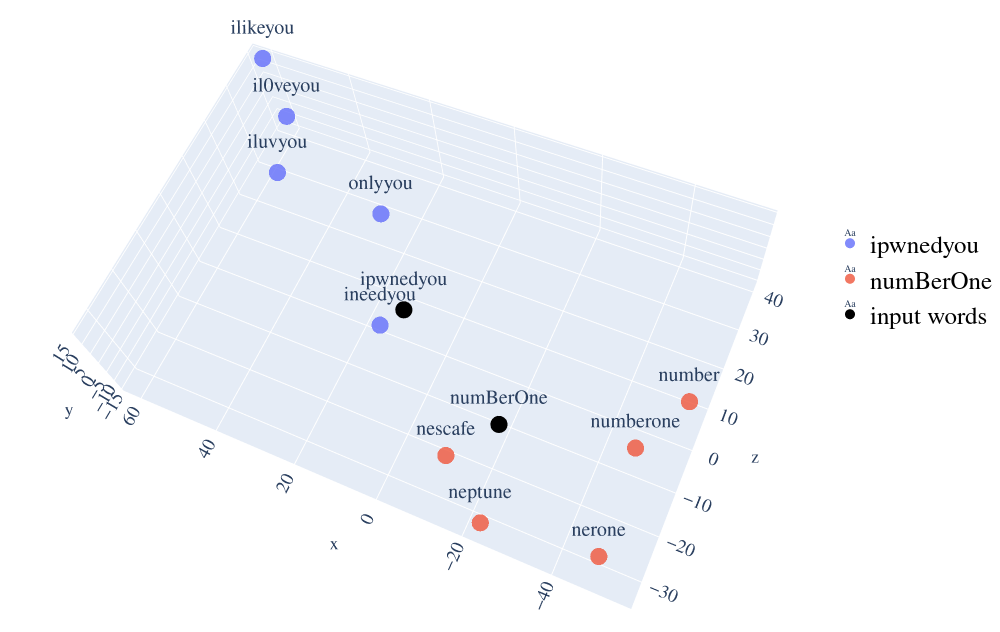
\includegraphics[width=15cm]{./immagini/3dplot.png}
    \caption{Grafico 3D per mostrare la similarità tra password}
    \label{3d}
\end{figure}
